\chapter{Mise en commun pour le projet}

Le but final de ces différents TD est de les rassembler pour obtenir une seule application Java permettant de taper au clavier en entrée une requête en langage naturel de type "Je veux tous les articles parlant de nanotechnologie" et d'obtenir les résultats de celle-ci les plus précis possibles en sortie.
Il est donc nécessaire de combiner en une seule interface :
\begin{itemize}
  \item la correction orthographique : tout d'abord 'tokenizer' notre phrase d'entrée à l'aide des lexiques de lemmes et des stop lists
  \item grammaire Antlr : transformer cette phrase simplifiée en une requête SQL et éventuellement la post-traiter pour en faire une requête SQL valide
  \item l'API Java pour PostgreSQL : cette interface Java/PostgreSQL doit enfin exécuter la requête SQL obtenue sur la base de données mise à disposition et retourner les résultats en sortie de manière exploitable pour éventuellement les afficher ensuite sur une page web
\end{itemize}

\java
Nous avons fait tout cela dans une class \lstinline{Main} qui contient la fonction \lstinline{main}. Cette fonction appelle des méthodes de l'ensemble des classes mentionnées plus haut afin d'appliquer les traitements dans le bon ordre, en commençant par demander une requête à l'utilisateur. Grâce à une boucle infinie s'arrêtant quand l'utilisateur entre une requête vide, nous sommes capables de ne pas interrompre le programme et de redemander autant de requêtes que l'utilisateur le souhaite.

\begin{figure}[H]
    \centering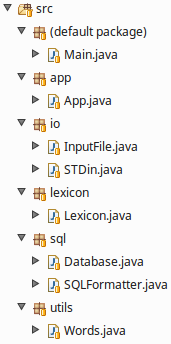
\includegraphics[width=0.25\textwidth]{images/projet.png}
    \caption{Ensemble du projet}
\end{figure}

Toutes les classes ont déjà été décrites dans ce rapport sauf trois :

\begin{itemize}
  \item \lstinline{App.java} : contient une constante utile à toutes les classes pour du debug, pour savoir quoi afficher dans la console :
      \java
        \begin{lstlisting}
public static final boolean DEBUG = true;
        \end{lstlisting}
  \item \lstinline{Words.java} : contient des méthodes \lstinline{static} pour nettoyer les différentes \lstinline{String} que nous manipulons (enlever les doubles espaces, faire des \lstinline{trim()}, etc.)
  \item \lstinline{SQLFormatter.java} : contient deux méthodes \lstinline{static}, nos pré et post-traitements
\end{itemize}

\medskip

Bien entendu, une fois toutes ces étapes réalisées, le travail de recherche n'est pas pour autant terminé car il peut être intéressant de prendre en compte les analyses sémantiques et pragmatiques par exemple, en plus de l'analyse syntaxique. Le nombre de requêtes en langage naturel possible étant potentiellement illimité, il est toujours possible de raffiner plus précisément le traitement de ces requêtes ; on peut par exemple avoir des requêtes portant sur plusieurs sujets différents, demandant des articles entre deux dates ou sur une période de temps, etc. Il sera intéressant d'essayer de perfectionner notre grammaire, le pré-traitement avec de donner la requête à la grammaire ainsi que le post-traitement, après avoir récupéré la sortie de la grammaire et avant d'exécuter la requête SQL.

\medskip

L'idée finale est d'obtenir une application parée à toute éventualité face à un utilisateur lambda qui est susceptible de demander n'importe quelle requête, portant sur n'importe quel sujet, à n'importe quelle date, etc.
